\documentclass[12pt, a4paper]{article}
\usepackage[utf8]{inputenc} 
\usepackage[magyar]{babel}
\usepackage[T1]{fontenc}


\usepackage{amssymb,amsmath,latexsym,amscd,tikz,url,hyperref, tikz-qtree, mathtools, cancel, amsthm, float, ulem, pgf, pgfplots}
\usepackage[mathscr]{eucal}
\usepackage{prftree}

\begin{document}
\section*{prftree usepackage}
 
\url{https://www.ctan.org/pkg/prftree}

\begin{displaymath}
 \prftree[r]{$\mathrm{Lam}_{(\prfref<assum:A>)}$}{
        \prftree[r]{$\mathrm{Lam}$}
        {\prfboundedassumption<assum:A>{x:A}}
        {\lambda y:B.x: B\to A}
    }
{\lambda x:A.\lambda y:B.x : A\to (B\to A)}
\end{displaymath}

\section*{tikz-qtree usepackage}

\url{https://ctan.org/pkg/tikz-qtree}

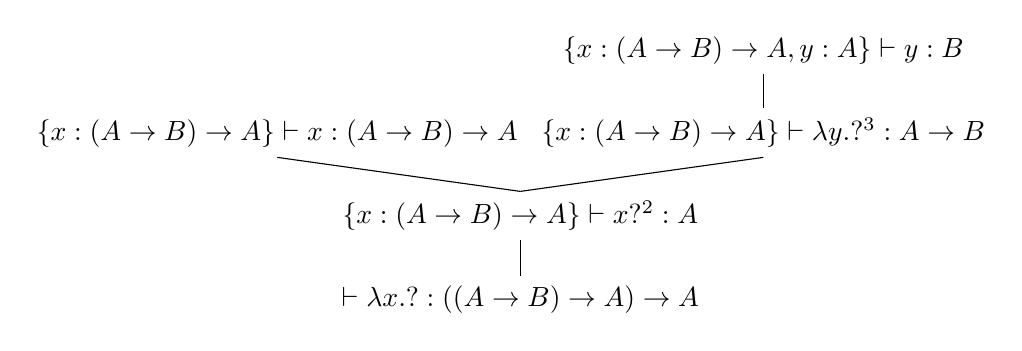
\begin{tikzpicture}[grow'=up]
            \Tree [.$\vdash \lambda x.?:((A\to B)\to A)\to A$ [.$\{x:(A\to B)\to A\}\vdash x?^2:A$ [.$\{x:(A\to B)\to A\}\vdash x:(A\to B)\to A$ ] [.$\{x:(A\to B)\to A\}\vdash\lambda y.?^3:A\to B$ [.$\{x:(A\to B)\to A,y:A\}\vdash y:B$ ] ] ] ]
\end{tikzpicture} 


\end{document}


